% LaTeX figure snippets. The writing-agent embeds these inline in main.tex.

% Figure 1: Framework schematic
\begin{figure}[htbp]
\centering

\includegraphics[width=0.92\textwidth]{figures/fig_framework.pdf}
\caption{Three representational strategies for encoding object identity in the
presence of non-identity variance. \textbf{Factorization} (left) places
non-identity variance along axes orthogonal to the identity subspace (orange
line), preserving non-identity information while maintaining a clean identity
readout. \textbf{Invariance} (middle) collapses non-identity variance into
compact regions that do not extend outside the identity subspace, discarding
non-identity information. \textbf{Entangled} codes (right) allow non-identity
variance to span directions overlapping the identity subspace, corrupting
identity decoding. Only factorization simultaneously preserves multiple
variables in a disentangled form.}
\label{fig:framework}
\end{figure}

% Figure 2: Simulation schematic
\begin{figure}[htbp]
\centering
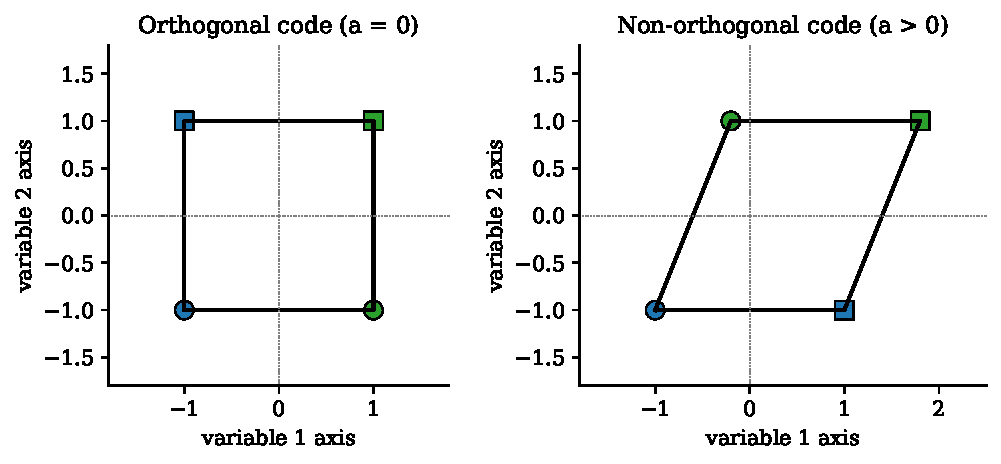
\includegraphics[width=0.82\textwidth]{figures/fig_simulation.pdf}
\caption{Simulation schematic for two binary variables encoded out of
\(N=10\) total dimensions. An orthogonal code (left; alignment \(a=0\)) forms
a square in the two-variable plane and supports accurate linear decoding of
both variables from few training samples under isotropic Gaussian noise. A
non-orthogonal code (right; alignment \(a>0\)) shears the square into a
parallelogram, preserving linear separability but degrading decoder
performance in the few-samples, noisy regime.}
\label{fig:simulation}
\end{figure}

% Figure 3: V4 to IT hierarchy schematic
\begin{figure}[htbp]
\centering
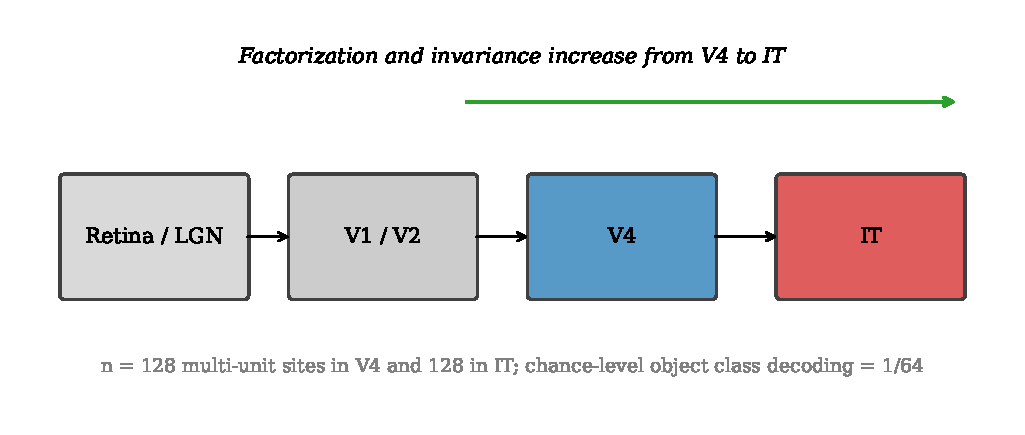
\includegraphics[width=0.92\textwidth]{figures/fig_hierarchy.pdf}
\caption{Schematic of the macaque ventral visual hierarchy and the empirical
trend reported in this work. Both factorization of object identity from
non-identity information and invariance to non-identity information increase
from V4 to IT in multi-unit recordings (\(n=128\) sites in V4 and 128 in IT;
chance object-class decoding accuracy \(=1/64\)). A representational lesion
that rotates the inter-class axes into the intra-class axes preserves mean
firing rates, covariance, and invariance while reducing factorization, and
significantly decreases object-class decoding accuracy in both areas.}
\label{fig:hierarchy}
\end{figure}

% Figure 4: Pipeline schematic
\begin{figure}[htbp]
\centering

\includegraphics[width=0.98\textwidth]{figures/fig_pipeline.pdf}
\caption{Evaluation pipeline for DNN brain-likeness. For each base scene
(\(n=100\)), we generate 10 parameter levels for each of four scene
parameters (object pose, background identity, lighting, camera viewpoint),
producing a 4000-image stimulus set. Each DNN (supervised, contrastive
self-supervised, or auxiliary self-supervised) produces layer-wise
representations from which factorization and invariance are computed using
the PCA-based or covariance-based metric. Model predictivity is evaluated
against 12 primate datasets spanning V4, IT/HVC, and behavior in macaques and
humans.}
\label{fig:pipeline}
\end{figure}
